% !TeX encoding = UTF-8
% !TeX program = pdflatex
% !TeX spellcheck = en_US
% !TEX root = main.tex

\documentclass[binding=0.6cm, Honours, english]{sapthesis}

\usepackage{microtype}
\usepackage[english]{babel}
\usepackage[utf8]{inputenx}
\usepackage[hyperfootnotes=false]{hyperref}
\usepackage[backend=biber,style=ieee,sorting=none]{biblatex}
\usepackage[titletoc]{appendix}
\usepackage{graphicx}
\graphicspath{ {./imgs/} }

\usepackage{nccmath}


\usepackage{caption,subcaption}

\usepackage{changepage}

\hypersetup{
	pdftitle={Encoders and IMU sensor fusion using the Kalman Filter},
	pdfauthor={Filippo Graziano},
	colorlinks  = true,
	urlcolor   = blue,
	linkcolor  = black,
	citecolor  = red
}

\addbibresource{07_bibliography.bib}

\renewcommand{\baselinestretch}{1.25} 

\usepackage{setspace}
\onehalfspacing

\makeatletter
\renewcommand\@makefntext[1]{\leftskip=2em\hskip-2em\@makefnmark#1}
\makeatother


\usepackage{listings}
\usepackage[dvipsnames]{xcolor}

\definecolor{deeppink}{rgb}{0.45, 0.00, 0.8}
\lstnewenvironment{ccode}[1][]{
	\lstset{
		language=C,
		numbers=left,
		stepnumber=1,
			tabsize=2,
		breaklines=true,
		basicstyle=\linespread{1.0}\ttfamily,
		keywordstyle=\color{blue}\ttfamily,
		stringstyle=\color{red}\ttfamily,
		commentstyle=\color{OliveGreen}\ttfamily,
		morecomment=[l][\color{deeppink}]{\#},
		columns=fullflexible,
		postbreak=\mbox{\textcolor{red}{$\hookrightarrow$}\space},
		escapeinside={(*@}{@*)},
		showstringspaces=false
	}
	\lstdefinestyle{nonumbers}
	{numbers=none}
}{}


\begin{document}

\title{Encoders and IMU sensor fusion \\using the Kalman Filter}

\author{Filippo Graziano}
\IDnumber{1761694}
\course{Computer and Control Engineering}
\courseorganizer{Faculty of Information Engineering, Informatics and Statistics}

\AcademicYear{2018/2019}
\copyyear{2019}

\advisor{Prof. Giorgio Grisetti}
\authoremail{graziano.1761694@studenti.uniroma1.it}

\frontmatter
\maketitle

%\dedication{To ...}

\begin{abstract}

In this thesis we will present the robot we have built in the last months. This robot implements two different localization algorithms:
\begin{itemize}
	\item on one side, it uses two encoders to measure the wheel rotations and estimate position and orientation using differential drive;
	\item on the other side, it uses an IMU\footnote{IMU stands for Inertial Measurement Unit} to estimate the position using inertial navigation.
\end{itemize}
The thesis is structured as follows:
\begin{itemize}
	\item Chapter 1 introduces the problem of localization and its importance for autonomous robots.
	\item Chapter 2 describes the sensors used by the robot and how they work.
	\item Chapter 3 includes a broad description of the robot, explaining the specific hardware used, the communication protocols needed, the firmware and how it interfaces with the sensors, and finally the host (i.e. the PC\footnote{PC stands for Portable Computer} interfacing with the firmware).
	\item Chapter 4 explains the two localization algorithms in detail.
	\item Chapter 5 provides some final considerations and hints possible improvements in the localization algorithms adopted for our robot.
	\item Some implementation details are provided in the Appendices.
\end{itemize}
The code for both the firmware running on the robot and the host is available at \url{https://github.com/FilippoGraziano98/Acquisition_Platform}.
\end{abstract}

%\begin{acknowledgments}

First, I would like to thank my parents, my sisters, my girlfriend and my closest friends for providing me with unfailing support and continuous encouragement throughout my years of study. This accomplishment would not have been possible without them.\\

I would also like to acknowledge my fellow students for making tough lessons less tiring and for stimulating me whenever my laziness was almost going to win me.\\

Finally, I express my sincere gratitude to my advisor Prof. Grisetti for his patience, guidance and insightful comments.
\end{acknowledgments}


\tableofcontents

\mainmatter
\chapter{Introduction}\label{intro_sensor_fusion}

Sensor fusion is a very important technique because almost all sensors have some limitations. It consists in combining sensory data derived from disparate sources such that the resulting information has less uncertainty than would be possible when using the single sources individually.\\

In our scenario we will combine different localization sensors, the encoders and the IMU. In this way each sensor will compensate for the weaknesses of the other and we will calculate a more accurate and robust odometry.\\

More in detail we will use Kalman filtering. This is an algorithm which takes measurements containing statistical noise and produces estimates of unknown variables (in our case we will estimate the position and the orientation of our robot) by updating a joint probability distribution over the variables in each timeframe.

Moreover the Kalman filter is the optimal filter for linear systems with Gaussian noise.

\chapter{Kalman Filter}
If there is no uncertainty we can model our system as described in following picture:
\begin{figure}[!ht]
	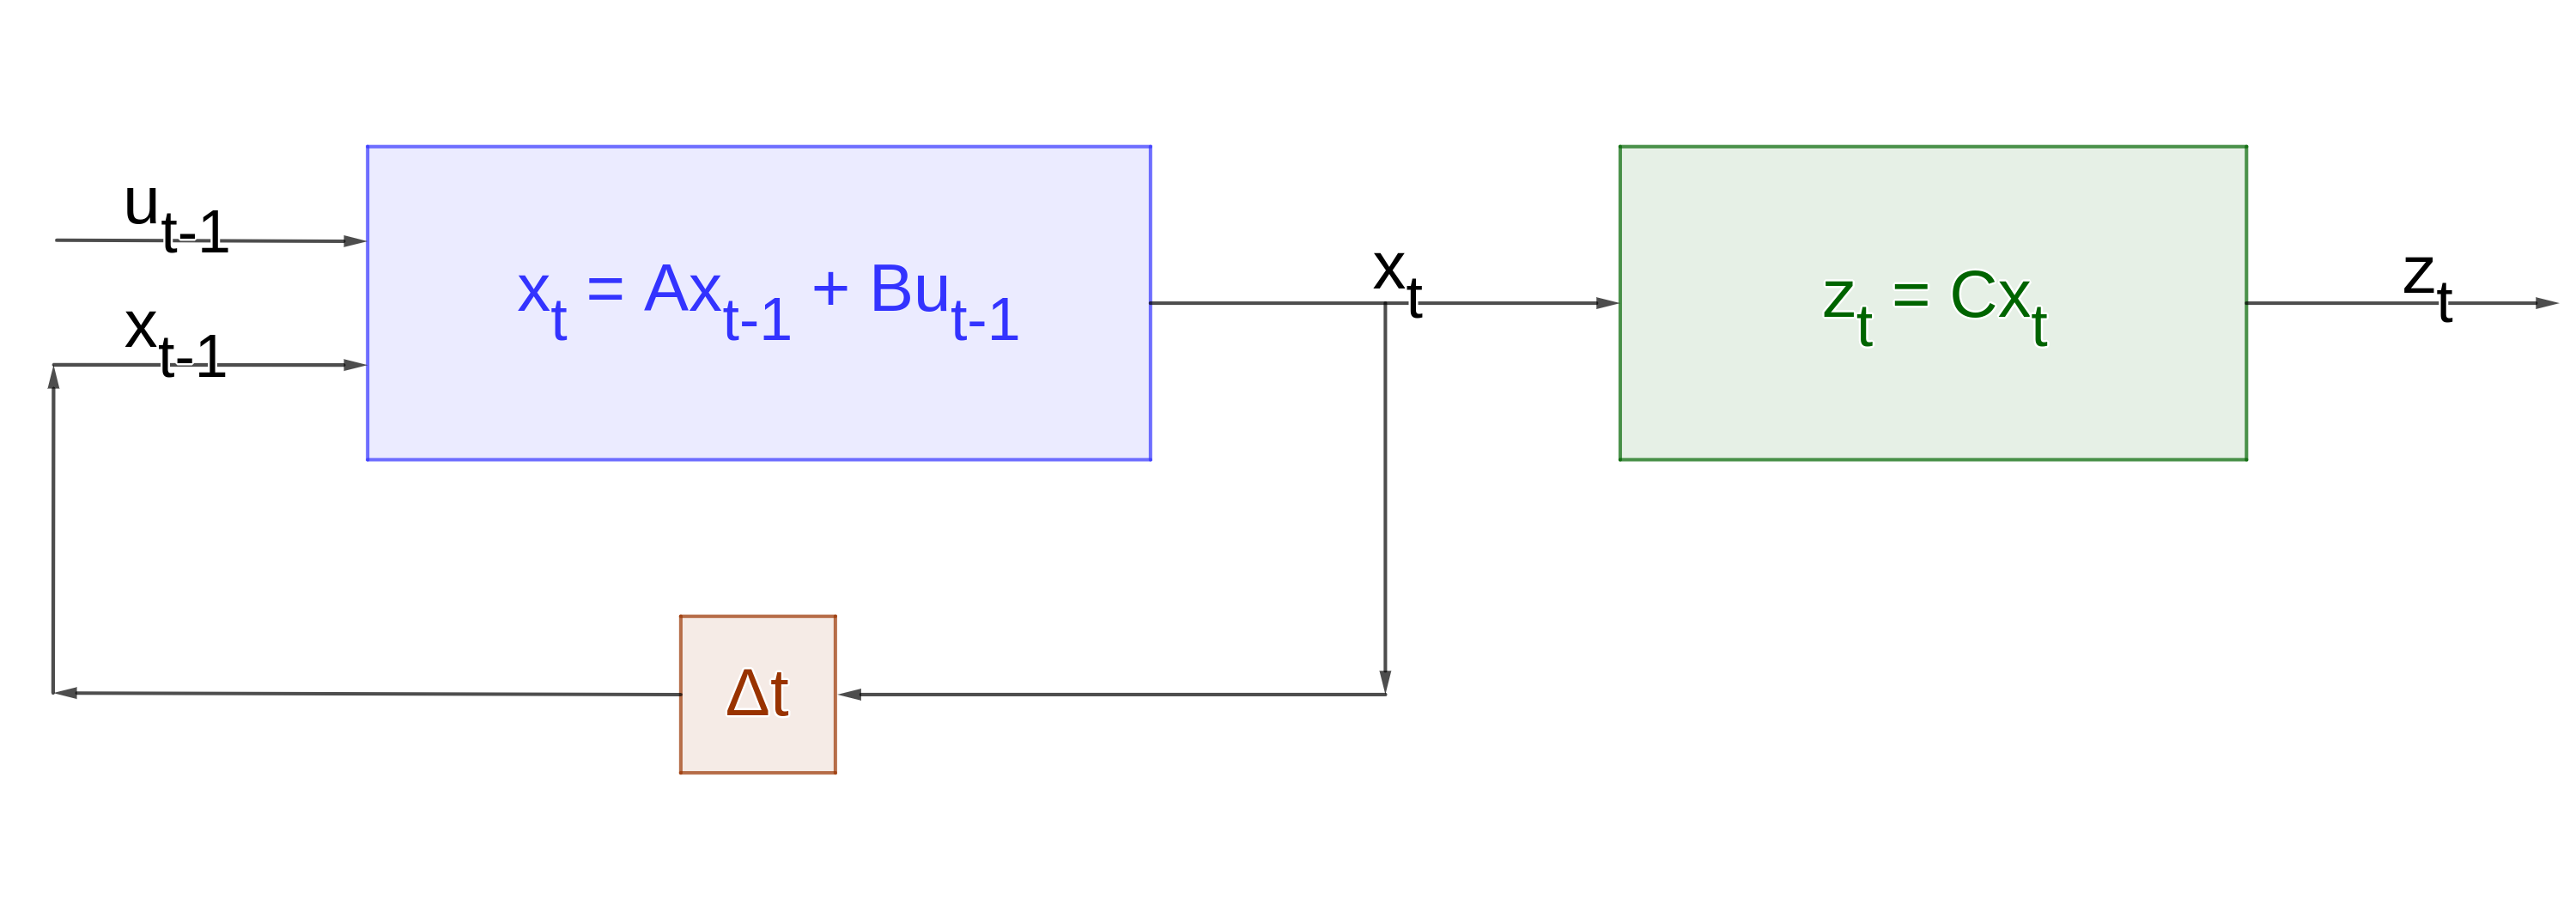
\includegraphics[scale=0.9]{system_model}
	\captionsetup{justification=centering, margin=1.5cm}
	\centering
	\caption{Deterministic System model.}
	\centering
\end{figure}
\begin{itemize}
	\item The state variables $x_t$ represents out robot's position and orientation.
	\item The control vector $u_t$ represents the rotational and translational accelerations our robot is subject to.
	\item The observation vector $z_t$ represents the sensors measurements.
\end{itemize}
As we can see in this model there is no uncertainty, the transition from a state to another is deterministic, we assume there is always no error in the observations or in the state.\\

However our inputs and our observations are not known with certainty. Therefore we must modify the previous model to include uncertainty and errors.
\begin{figure}[!ht]
	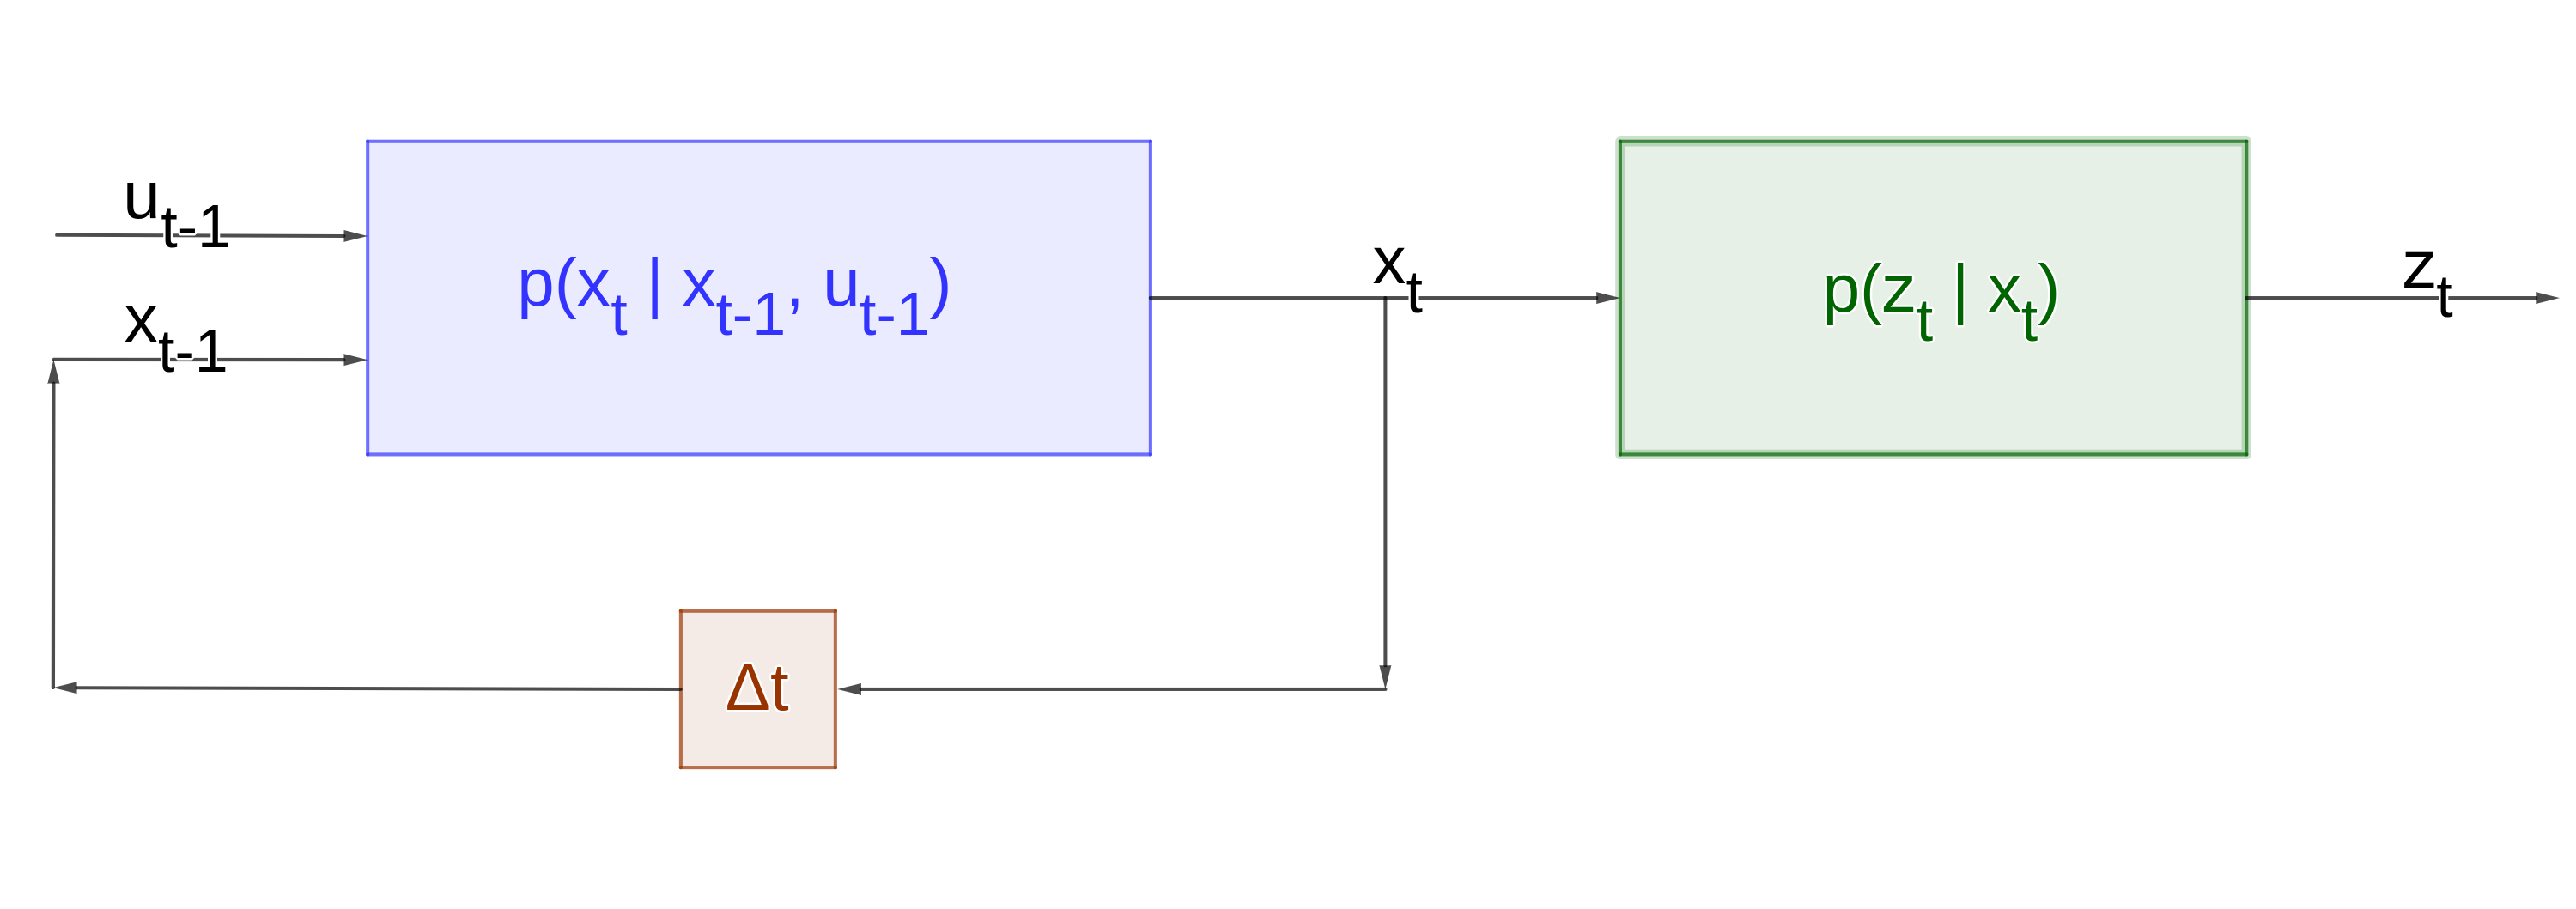
\includegraphics[scale=0.9]{stochastic_system_model}
	\captionsetup{justification=centering, margin=1.5cm}
	\centering
	\caption{Stochastic System model.}
	\centering
\end{figure}
\begin{itemize}
	\item $p(x_t | x_{t-1}, u_{t-1})$ is the transition model, which correlates the current state with the previous state and the previous control.
	\item $p(z_t | x_t)$ is the observation model, which correlates the current observation with the current state.
\end{itemize}

The goal of the Kalman filter is to compute the distribution over the current state given the sequence of all controls and of all observations up to the current instant, i.e. $p(x_t | u_{0:t-1}, z_{0:t})$.

As a basic idea we will perform two successive phases at each time instant, a predict phase and an update one.
\begin{itemize}
	\item In the predict phase we only consider the previous state and control to update the state. Therefore we will calculate the expected state in consequence to the control we gave to the system.
	\item In the update phase we update the state according to what we have observed and to how likely it is to have these observations from the current state.
\end{itemize}

In particular, in Kalman filtering we assume the state and the noise to be Gaussian. Since Gaussian distributions are closed under affine transformation, chain rule, marginalization and conditioning the state will always remain a Gaussian distribution. Therefore in each phase we will just have to compute the new parameters of the Gaussian.

In the following we will briefly present the Kalman filtering algorithm. For further details about Kalman Filtering we recommend the slides of the "Probabilistic Robotics" Course, held by Prof. Giorgio Grisetti at Sapienza University of Rome\supercite{prob_rob}.

\section{Predict phase}
In the predict phase we update the estimated state incorporating the latest control. The transition model is an affine transformation of the state and the control:
\begin{align}
	x_t = A_t x_{t-1} + B_t u_{t-1}\label{pred_model}
\end{align}
The previous state $x_{t-1}$ is a Gaussian with mean $\mu_{t-1|t-1}$ and covariance $\Sigma_{t-1|t-1}$.
While the control vector $u_{t-1}$ is a Gaussian with mean $\mu_{u,t-1}$ and covariance $\Sigma_{u,t-1}$.

After the predict phase, the estimated state $p(x_{t|t-1})$ is still a Gaussian, with the following parameters:
\begin{align}
	\mu_{t|t-1} &= A_t \mu_{t-1|t-1} + B_t \mu_{u,t-1}\label{pred_mean}\\
	\Sigma_{t|t-1} &= A_t \Sigma_{t-1|t-1} A_t^T + B_t \Sigma_{u,t-1} B_t^T\label{pred_cov}
\end{align}

\section{Update phase}
In the update phase we incorporate the new observations in the state estimate, starting form the observation model:
\begin{align}
	z_t = C_t x_{t|t-1}\label{upd_model}
\end{align}

We want to compute the probability $p(x_t|z_t)$ given the following distributions:
\begin{itemize}
	\item $p(z_t|x_t)$ which is a Gaussian distribution with mean $\mu_{z,t} = C_t x_{t|t-1}$ and covariance $\Sigma_{z,t}$,
	\item $p(x_{t|t-1})$ which is the Gaussian distribution of the estimated state after the predict phase.
\end{itemize}

In the update phase we compute the Kalman gain:
\begin{align}
	K_t = \Sigma_{t|t-1} C_t^T (\Sigma_{z,t} + C_t \Sigma_{t|t-1} C_t^T)^{-1}\label{kalman_gain}
\end{align}

Using the Kalman gain we can update the parameters of the Gaussian distribution representing the state:
\begin{align}
	\mu_{t|t} &= \mu_{t|t-1} + K_t (z_t - \mu_{z,t})\\
	\Sigma_{t|t} &= (I - K_t C_t) \Sigma_{t|t-1}
\end{align}

\paragraph{Role of the observation covariance}
We can rewrite the \ref{kalman_gain} as follows:
\begin{gather*}
	K_t = \frac{\Sigma_{t|t-1} C_t^T}{\Sigma_{z,t} + C_t \Sigma_{t|t-1} C_t^T}
\end{gather*}
In this form it becomes evident the role of the observation covariance $\Sigma_{z,t}$ in the update phase.\\

If the observation covariance (i.e. the observation uncertainty) tends to zero, then the Kalman Gain tends to:
\begin{gather*}
	K_t = \frac{\Sigma_{t|t-1} C_t^T}{C_t \Sigma_{t|t-1} C_t^T} = \frac{1}{C_t}	
\end{gather*}
and consequently:
\begin{align*}
	\mu_{t|t} &= \mu_{t|t-1} + K_t (z_t - \mu_{z,t}) = \mu_{t|t-1} + \frac{1}{C_t} (z_t - C_t \mu_{t|t-1}) =\nonumber\\
			&= \mu_{t|t-1} + \frac{1}{C_t} z_t - \mu_{t|t-1} = C_t^{-1}z_t\\
	\Sigma_{t|t} &= (I - K_t C_t) \Sigma_{t|t-1} = (I - \frac{1}{C_t} C_t) \Sigma_{t|t-1} = (I - I) \Sigma_{t|t-1} = 0
\end{align*}
Therefore if the observation uncertainty tends to zero, the state estimate can be calculated only from the current observation and will have zero covariance.\\

If the observation covariance tends to infinity, then the Kalman Gain tends to zero and consequently:
\begin{gather*}
	K_t = \frac{\Sigma_{t|t-1} C_t^T}{\Sigma_{z,t} + C_t \Sigma_{t|t-1} C_t^T} = 0
\end{gather*}
\begin{align*}
	\mu_{t|t} &= \mu_{t|t-1} + K_t (z_t - \mu_{z,t}) = \mu_{t|t-1}\\
	\Sigma_{t|t} &= (I - K_t C_t) \Sigma_{t|t-1} = \Sigma_{t|t-1}
\end{align*}
Therefore if the observation uncertainty tends to infinity, the state estimate will not be updated by the observations.\\

Wrapping up, if the observation covariance tends to zero, the state estimate will move immediately on the observations; while if the covariance tends to infinity the state estimate will not incorporate the observations.


\chapter{Kalman Filter design for our robot}
Since the 16 MHz CPU on the MEGA2560 board was not able to carry out all the matrix calculations required by the Kalman filter at 100 Hz, we have decided to do all the computations host-side using the 2.7 GHz CPU on our PC\footnote{PC stands for Portable Computer} and send the observations via UART from the robot at 100 Hz.\\

In order to use the Kalman filter presented in the previous chapter, we only have to decide how to model our problem. More in detail we must:
\begin{itemize}
	\item choose how to represent the state,
	\item choose how to represent the controls,
	\item implement a transition model,
	\item choose how to represent the observations,
	\item implement an observation model.
\end{itemize}

Our implementation of the filter is shown in Appendix \ref{kf_implementation}.

\section{Predict phase}

\subsection{State vector}\label{state}
Our state must represent all the information on the position and orientation of the robot. Therefore we have used an 8-components state:
\begin{itemize}
	\item x representing the global displacement along the x-axis,
	\item $\dot{x}$ representing the translational velocity along the global x-axis,
	\item $\ddot{x}$ representing the translational acceleration along the global x-axis,
	\item y representing the global displacement along the y-axis,
	\item $\dot{y}$ representing the translational velocity along the global y-axis,
	\item $\ddot{y}$ representing the translational acceleration along the global y-axis,
	\item $\theta$ representing the global orientation along the z-axis,
	\item $\dot{\theta}$ representing the rotational velocity along the global z-axis.
\end{itemize}
We have included the translational accelerations because our accelerometers measure accelerations, instead we have stopped to rotational velocities because this is what our gyroscope measures.\\

Since our state will be represented by a Gaussian distribution we need to initialize both its mean and its covariance. We have decided to initialize them both with zeros because we want to measure the displacement from the starting position and because there is no uncertainty at the beginning.

\subsection{Controls vector}\label{controls}
Since our robot is pushed by hand (having no motors), we have no knowledge about the controls vector. However we will use this vector to model noise in the transition process and to introduce uncertainty in it; therefore we will assume the control vector to be zero-mean but with non-zero covariance.\\

We will use the controls vector to model spikes in the translational accelerations or in the rotational velocity which could not be observed.
\begin{itemize}
	\item $\dddot{x}$ representing a derivative of the translational acceleration along the global x-axis,
	\item $\dddot{y}$ representing a derivative of the translational acceleration along the global y-axis,
	\item $\ddot{\theta}$ representing a derivative of the rotational velocity (i.e. a rotational acceleration) along the global z-axis.
\end{itemize}

We will use the following covariance matrix:
\begin{align}
	\Sigma_u = \begin{pmatrix}
				0.1 & 0 & 0\\
				0 & 0.1 & 0\\
				0 & 0 & 0.5\\
			\end{pmatrix}
\end{align}

We need high control covariances because, since we are pushing the robot by hand, our process is very noisy; surely if we had engines controlling the robot's wheels the process would be more continuous and we could use lower covariances.

\subsection{Transition model}
We are now ready to implement the transition model, which will be used in the Predict phase. In order to define the affine transformation \ref{pred_model}, we must define the state transition matrix $A_t$ and the input matrix $B_t$.\\

According to how we defined the state in section \ref{state} and to some basics of kinematics\footnote{Basic kinematic relationships between position, velocity and acceleration:\begin{fleqn}\begin{equation}x = x + \dot{x} \Delta t + .5 \ddot{x} \Delta t^2\nonumber\end{equation}\begin{equation}\dot{x} = \dot{x} + \ddot{x} \Delta t\nonumber\end{equation}\end{fleqn}}, we can define the following state transition matrix:
\begin{align}
	A = \begin{pmatrix}
				1 & \Delta t & .5 \Delta t^2 & 0 & 0 & 0 & 0 & 0\\
				0 & 1 & \Delta t & 0 & 0 & 0 & 0 & 0\\
				0 & 0 & 1 & 0 & 0 & 0 & 0 & 0\\
				0 & 0 & 0 & 1 & \Delta t & .5 \Delta t^2 & 0 & 0\\
				0 & 0 & 0 & 0 & 1 & \Delta t & 0 & 0\\
				0 & 0 & 0 & 0 & 0 & 1 & 0 & 0\\
				0 & 0 & 0 & 0 & 0 & 0 & 1 & \Delta t\\
				0 & 0 & 0 & 0 & 0 & 0 & 0 & 1\\
			\end{pmatrix}
\end{align}

According to how we have defined the controls vector in section \ref{controls} we can define the following input matrix:
\begin{align}
	B = \begin{pmatrix}
				.167 \Delta t^3 & 0 & 0\\
				.5 \Delta t^2 & 0 & 0\\
				\Delta t & 0 & 0\\
				0 & .167 \Delta t^3 & 0\\
				0 & .5 \Delta t^2 & 0\\
				0 & \Delta t & 0\\
				0 & 0 & .167 \Delta t^3\\
				0 & 0 & .5 \Delta t^2\\
				0 & 0 & \Delta t\\
			\end{pmatrix}
\end{align}

We can notice how this two matrices are independent of the precise current sampling instant and they remain constant throughout all the computation.\\

From the equations \ref{pred_mean} and \ref{pred_cov}, remembering that our control is zero-mean we obtain the following predict phase equations:
\begin{align}
	\mu_{t|t-1} &= A \mu_{t-1|t-1}\\
	\Sigma_{t|t-1} &= A \Sigma_{t-1|t-1} A^T + B \Sigma_{u,t-1} B^T
\end{align}


\section{Update phase}
\subsection{IMU observations}
\subsubsection{IMU observations vector}
The accelerometer gives us measurements about the accelerations along the three axes, while the gyroscope measures rotational velocities along the three axes. Assuming that our robot moves only in 2D we will consider only:
\begin{itemize}
	\item $\ddot{x}_z$ which is the translational acceleration along the x-axis measured by the accelerometer,
	\item $\ddot{y}_z$ which is the translational acceleration along the y-axis measured by the accelerometer,
	\item $\dot{\theta}_z$ which is the rotational velocity along the z-axis measured by the gyroscope.
\end{itemize}

We will consider these measurements as independent, therefore the IMU covariance matrix will be diagonal. Moreover since the accelerometer is very noisy and inaccurate, we will give the accelerometer observations a relevant covariance, instead since the gyroscope is much less noisy we will give it less covariance.
\begin{align}
	\Sigma_{IMU} = \begin{pmatrix}
				0.1 & 0 & 0\\
				0 & 0.1 & 0\\
				0 & 0 & 0.000001\\
			\end{pmatrix}
\end{align}
Let us note how the measurement error covariances were defined by trial and error since they were not provided by the IMU manufacturer.

\subsubsection{IMU observation model}
To define the observation model for the IMU observations, we must define only the observation matrix $C_t$ to be used in the equation \ref{upd_model}.
\begin{align}
	C_{IMU} = \begin{pmatrix}
				0 & 0 & 1 & 0 & 0 & 0 & 0 & 0\\
				0 & 0 & 0 & 0 & 0 & 1 & 0 & 0\\
				0 & 0 & 0 & 0 & 0 & 0 & 0 & 1\\
			\end{pmatrix}
\end{align}



\subsection{Encoders observations}
Unlike the IMU which gives us measurements for which the definition of an observation matrix is immediate, the encoders measures the wheel rotations.\\

\subsubsection{Linearized Observation Matrix}
We have started considering the wheels rotations as the observations to be used in Kalman filter. Since we assume the encoders to be very accurate we assumed these measurements to have small covariance.
\begin{align}
	\Sigma_{encoders,linearized} = \begin{pmatrix}
				0.0000001 & 0\\
				0 & 0.0000001\\
			\end{pmatrix}
\end{align}
Let us note how these measurement error covariances were defined by trial and error since they were not provided by the encoders manufacturer.

\begin{figure}[!ht]
	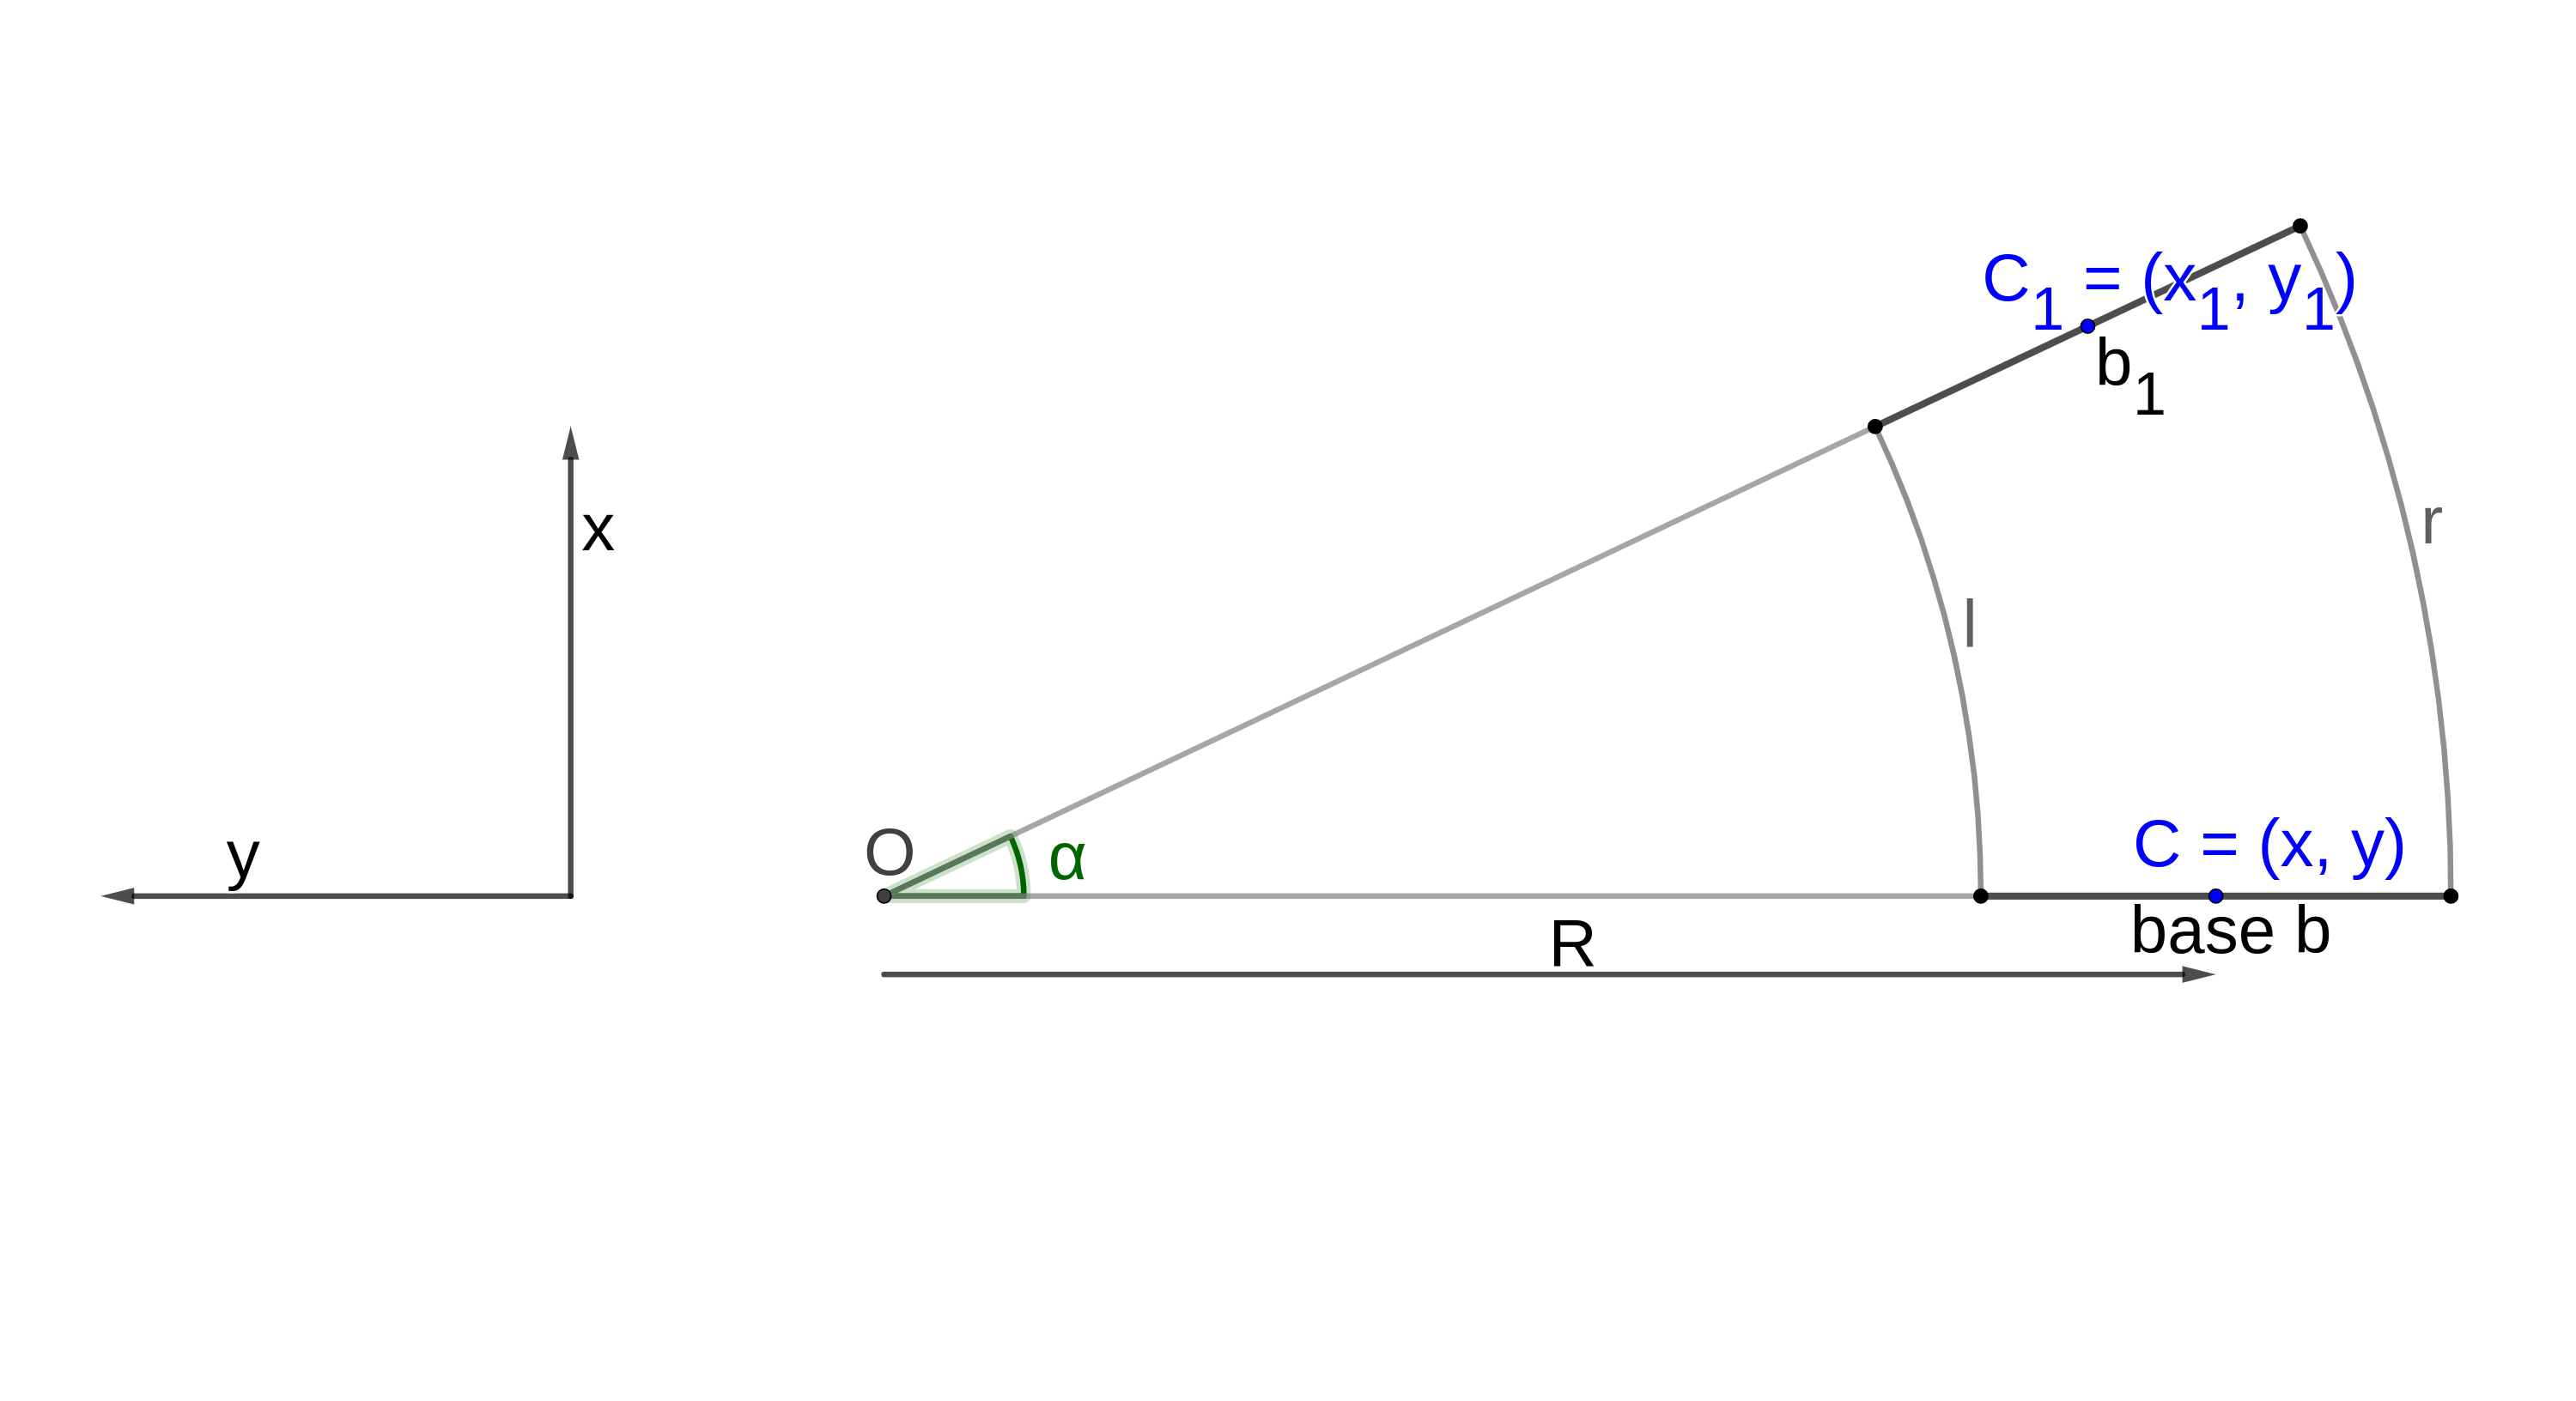
\includegraphics[scale=0.9]{differential_drive_1}
	\captionsetup{justification=centering, margin=1.5cm}
	\centering
	\caption{Model of an instantaneous movement through a rotation.}
	\centering
\end{figure}

As described in my thesis\supercite{Graziano:BscThesis:2019}, the rotations of the left and right wheel (\textit{l} and \textit{r} respectively) are related to the parameters of the local rotation (the radius \textit{R} and the angle $\Delta \theta$) by the equations (where \textit{b} is the length of the wheel axis):
\begin{align}
	r &= (R + b/2) \Delta \theta\label{r}\\
	l &= (R - b/2) \Delta \theta\label{l}
\end{align}

Moreover \textit{R} is related to the local movement by the equation:
\begin{align}
	\Delta x_{local} = R \sin\Delta \theta\label{x_local_r}
\end{align}

and the local movement can be related to the global movement using:
\begin{align}
	\Delta x_{local} = \Delta x \cos\theta + \Delta y \sin\theta\label{x_local_global}
\end{align}

Therefore using the \ref{x_local_r} and the \ref{x_local_global}:
\begin{align}
	R = \frac{\Delta x_{local}}{\sin\Delta \theta} = \frac{\Delta x \cos\theta + \Delta y \sin\theta}{\sin\Delta \theta}\label{R}
\end{align}

Finally using the \ref{r}, the \ref{l} and the \ref{R}:
\begin{align}
	r &= (\frac{\Delta x \cos\theta + \Delta y \sin\theta}{\sin\Delta \theta} + b/2) \Delta \theta\\
	l &= (\frac{\Delta x \cos\theta + \Delta y \sin\theta}{\sin\Delta \theta} - b/2) \Delta \theta
\end{align}

These equations enable us to calculate the observations starting from the state, however these equations are not linear. Therefore we have linearized them using the Taylor expansion to the first order centered in zero\footnote{The Taylor expansion to the first order for a function $f(x,y)$ results in the polynomial:\begin{gather*}P = f(0,0) + \der{f(0,0)}{x} x + \der{f(0,0)}{y} y\end{gather*}}.
\begin{align}
	r &= \cos\theta \Delta x + \sin\theta \Delta y + \frac{b}{2}\Delta \theta\label{r_lin}\\
	l &= \cos\theta \Delta x + \sin\theta \Delta y - \frac{b}{2}\Delta \theta\label{l_lin}
\end{align}

In order to use these equations in the observation matrix we must write $\Delta x$, $\Delta y$, $\Delta \theta$ as a function of the state:
\begin{align}
	\Delta x &= \dot{x} \Delta t + \frac{1}{2} \ddot{x} \Delta t\label{dx}\\
	\Delta y &= \dot{y} \Delta t + \frac{1}{2} \ddot{y} \Delta t\label{dy}\\
	\Delta \theta &= \dot{\theta} \Delta t\label{dtheta}
\end{align}

Using the \ref{r_lin}, the \ref{l_lin}, the \ref{dx}, the \ref{dy} and the \ref{dtheta}:
\begin{align}
	r &= (\cos\theta \Delta t)\dot{x} + (.5 \cos\theta \Delta t^2)\ddot{x} + (\sin\theta \Delta t)\dot{y} + (.5 \sin\theta \Delta t^2)\ddot{y} + (.5 b \Delta t)\dot{\theta}\\
	l &= (\cos\theta \Delta t)\dot{x} + (.5 \cos\theta \Delta t^2)\ddot{x} + (\sin\theta \Delta t)\dot{y} + (.5 \sin\theta \Delta t^2)\ddot{y} - (.5 b \Delta t)\dot{\theta}
\end{align}

Now we are ready to write the linearized observation matrix:
\begin{align}
	C_{encoders,linearized} = \begin{pmatrix}
				0 & \cos\theta \Delta t & .5 \cos\theta \Delta t^2 & 0 & \sin\theta \Delta t & .5 \sin\theta \Delta t^2 & 0 & .5 b \Delta t\\
				0 & \cos\theta \Delta t & .5 \cos\theta \Delta t^2 & 0 & \sin\theta \Delta t & .5 \sin\theta \Delta t^2 & 0 & -.5 b \Delta t\\
			\end{pmatrix}
\end{align}

However in this matrix all the dependencies from $y$, $\dot{y}$, $\ddot{y}$ are functions of $\sin\theta$. Since we start with our robot in motionless state with orientation corresponding to $\theta = 0$ (and since $\sin 0 = 0$), we will have zero components in the observation matrix for all the components relative to the motion along the y-axis, therefore the update phase will not reduce the uncertainty relative to these components as it does for the ones relative to the motion along the x-axis. This leads to high uncertainty on the y-axis even if the robot is stationary and we observe no wheel rotations. This is certainly a non-desirable effect.

\subsubsection{Converted Measurements Observation Matrix}
In order to solve the problem previously described, we have changed our approach to the encoders measurements. This time we have not considered as observations directly the wheel rotations, but we converted the wheel rotations in the local instant movement and used this movement as the observation.\\

As described in my thesis\supercite{Graziano:BscThesis:2019} we can calculate the local movement using the Differential Drive technique:
\begin{align}
	\Delta x &= \frac{r + l}{2} \frac{\sin \Delta\theta}{\Delta\theta}\\
	\Delta y &= \frac{r + l}{2} \frac{1 - \cos \Delta\theta}{\Delta\theta}\\
	\Delta\theta &= \frac{r - l}{b}
\end{align}

Since we assume the encoders to be very accurate, we can still believe these observations as reliable. However we must point out that the encoders are subject to errors when the wheels start to slip; in this case the highest drift will be seen in the orientation because calculating $\Delta x$, $\Delta y$ we use the mean between \textit{r} and \textit{l} while updating $\Delta\theta$ we use the difference between the two wheels rotations. Therefore we will give a slightly higher covariance to $\Delta\theta$.
\begin{align}
	\Sigma_{encoders,converted} = \begin{pmatrix}
				0.0000001 & 0 & 0\\
				0 & 0.0000001 & 0\\
				0 & 0 & 0.000001
			\end{pmatrix}
\end{align}

Using the local movement $\Delta\theta$, $\Delta x$, $\Delta y$ as the observation, we can define the observation matrix as follows.
\begin{align}
	\Delta x_{local} &= \Delta x \cos\theta + \Delta y \sin\theta\\
	\Delta y_{local} &= -\Delta x \sin\theta + \Delta y \cos\theta\\
	\Delta\theta_{local} &= \Delta\theta
\end{align}

Using again the \ref{dx}, the \ref{dy} and the \ref{dtheta}, we can rewrite the previous equations as follows:
\begin{align}
	\Delta x_{local} &= (\cos\theta \Delta t)\dot{x} + (.5 \cos\theta \Delta t^2)\ddot{x} + (\sin\theta \Delta t)\dot{y} + (.5 \sin\theta \Delta t^2)\ddot{y}\\
	\Delta y_{local} &= (-\sin\theta \Delta t)\dot{x} + (-.5 \sin\theta \Delta t^2)\ddot{x} + (\cos\theta \Delta t)\dot{y} + (.5 \cos\theta \Delta t^2)\ddot{y}\\
	\Delta\theta_{local} &= \dot{\theta} \Delta t
\end{align}
Finally we can write the converted measurements observation matrix:
\begin{align}
	C_{encoders,converted} = \begin{pmatrix}
				0 & \cos\theta \Delta t & .5 \cos\theta \Delta t^2 & 0 & \sin\theta \Delta t & .5 \sin\theta \Delta t^2 & 0 & 0\\
				0 & -\sin\theta \Delta t & -.5 \sin\theta \Delta t^2 & 0 & \cos\theta \Delta t & .5 \cos\theta \Delta t^2 & 0 & 0\\
				0 & 0 & 0 & 0 & 0 & 0 & 0 & \Delta t\\
			\end{pmatrix}
\end{align}

\subsection{Joint Update phase}
Since we are sampling both the sensors at the same rate (100 Hz), we will consider a single observation vector:
\begin{itemize}
	\item $\ddot{x}_z$ which is the translational acceleration along the x-axis measured by the accelerometer,
	\item $\ddot{y}_z$ which is the translational acceleration along the y-axis measured by the accelerometer,
	\item $\dot{\theta}_z$ which is the rotational velocity along the z-axis measured by the gyroscope,
	\item $\Delta x_{local}$ which is the local displacement along the x-axis calculated from the encoders rotations,
	\item $\Delta y_{local}$ which is the local displacement along the y-axis calculated from the encoders rotations,
	\item $\Delta \theta_{local}$ which is the local orientation change calculated from the encoders rotations.
\end{itemize}

Globally the observation covariance will be:
\begin{align}
	\Sigma_z = \begin{pmatrix}
				0.1 & 0 & 0 & 0 & 0 & 0\\
				0 & 0.1 & 0 & 0 & 0 & 0\\
				0 & 0 & 0.000001 & 0 & 0 & 0\\
				0 & 0 & 0 & 0.0000001 & 0 & 0\\
				0 & 0 & 0 & 0 & 0.0000001 & 0\\
				0 & 0 & 0 & 0 & 0 & 0.000001\\
			\end{pmatrix}
\end{align}
and the observation matrix will be:
\begin{align}
	C_t = \begin{pmatrix}
				0 & 0 & 1 & 0 & 0 & 0 & 0 & 0\\
				0 & 0 & 0 & 0 & 0 & 1 & 0 & 0\\
				0 & 0 & 0 & 0 & 0 & 0 & 0 & 1\\
				0 & \cos\theta \Delta t & .5 \cos\theta \Delta t^2 & 0 & \sin\theta \Delta t & .5 \sin\theta \Delta t^2 & 0 & 0\\
				0 & -\sin\theta \Delta t & -.5 \sin\theta \Delta t^2 & 0 & \cos\theta \Delta t & .5 \cos\theta \Delta t^2 & 0 & 0\\
				0 & 0 & 0 & 0 & 0 & 0 & 0 & \Delta t\\
			\end{pmatrix}
\end{align}
We can notice how this matrix depends on the current sampling instant, in particular it depends on the current orientation. Therefore we will need to recalculate the observation matrix at each iteration of the filter.

\chapter{Conclusions}

In this report we have presented the Kalman filter we used for our robot. Now we will report an evaluation test on the accuracy af the filter with respect to the odometries calculated using sensors individually.\\

We drove the robot along the following trajectory starting and ending at point A and passing through the other points in the order B, C, D, E ,F.
\begin{figure}[!ht]
	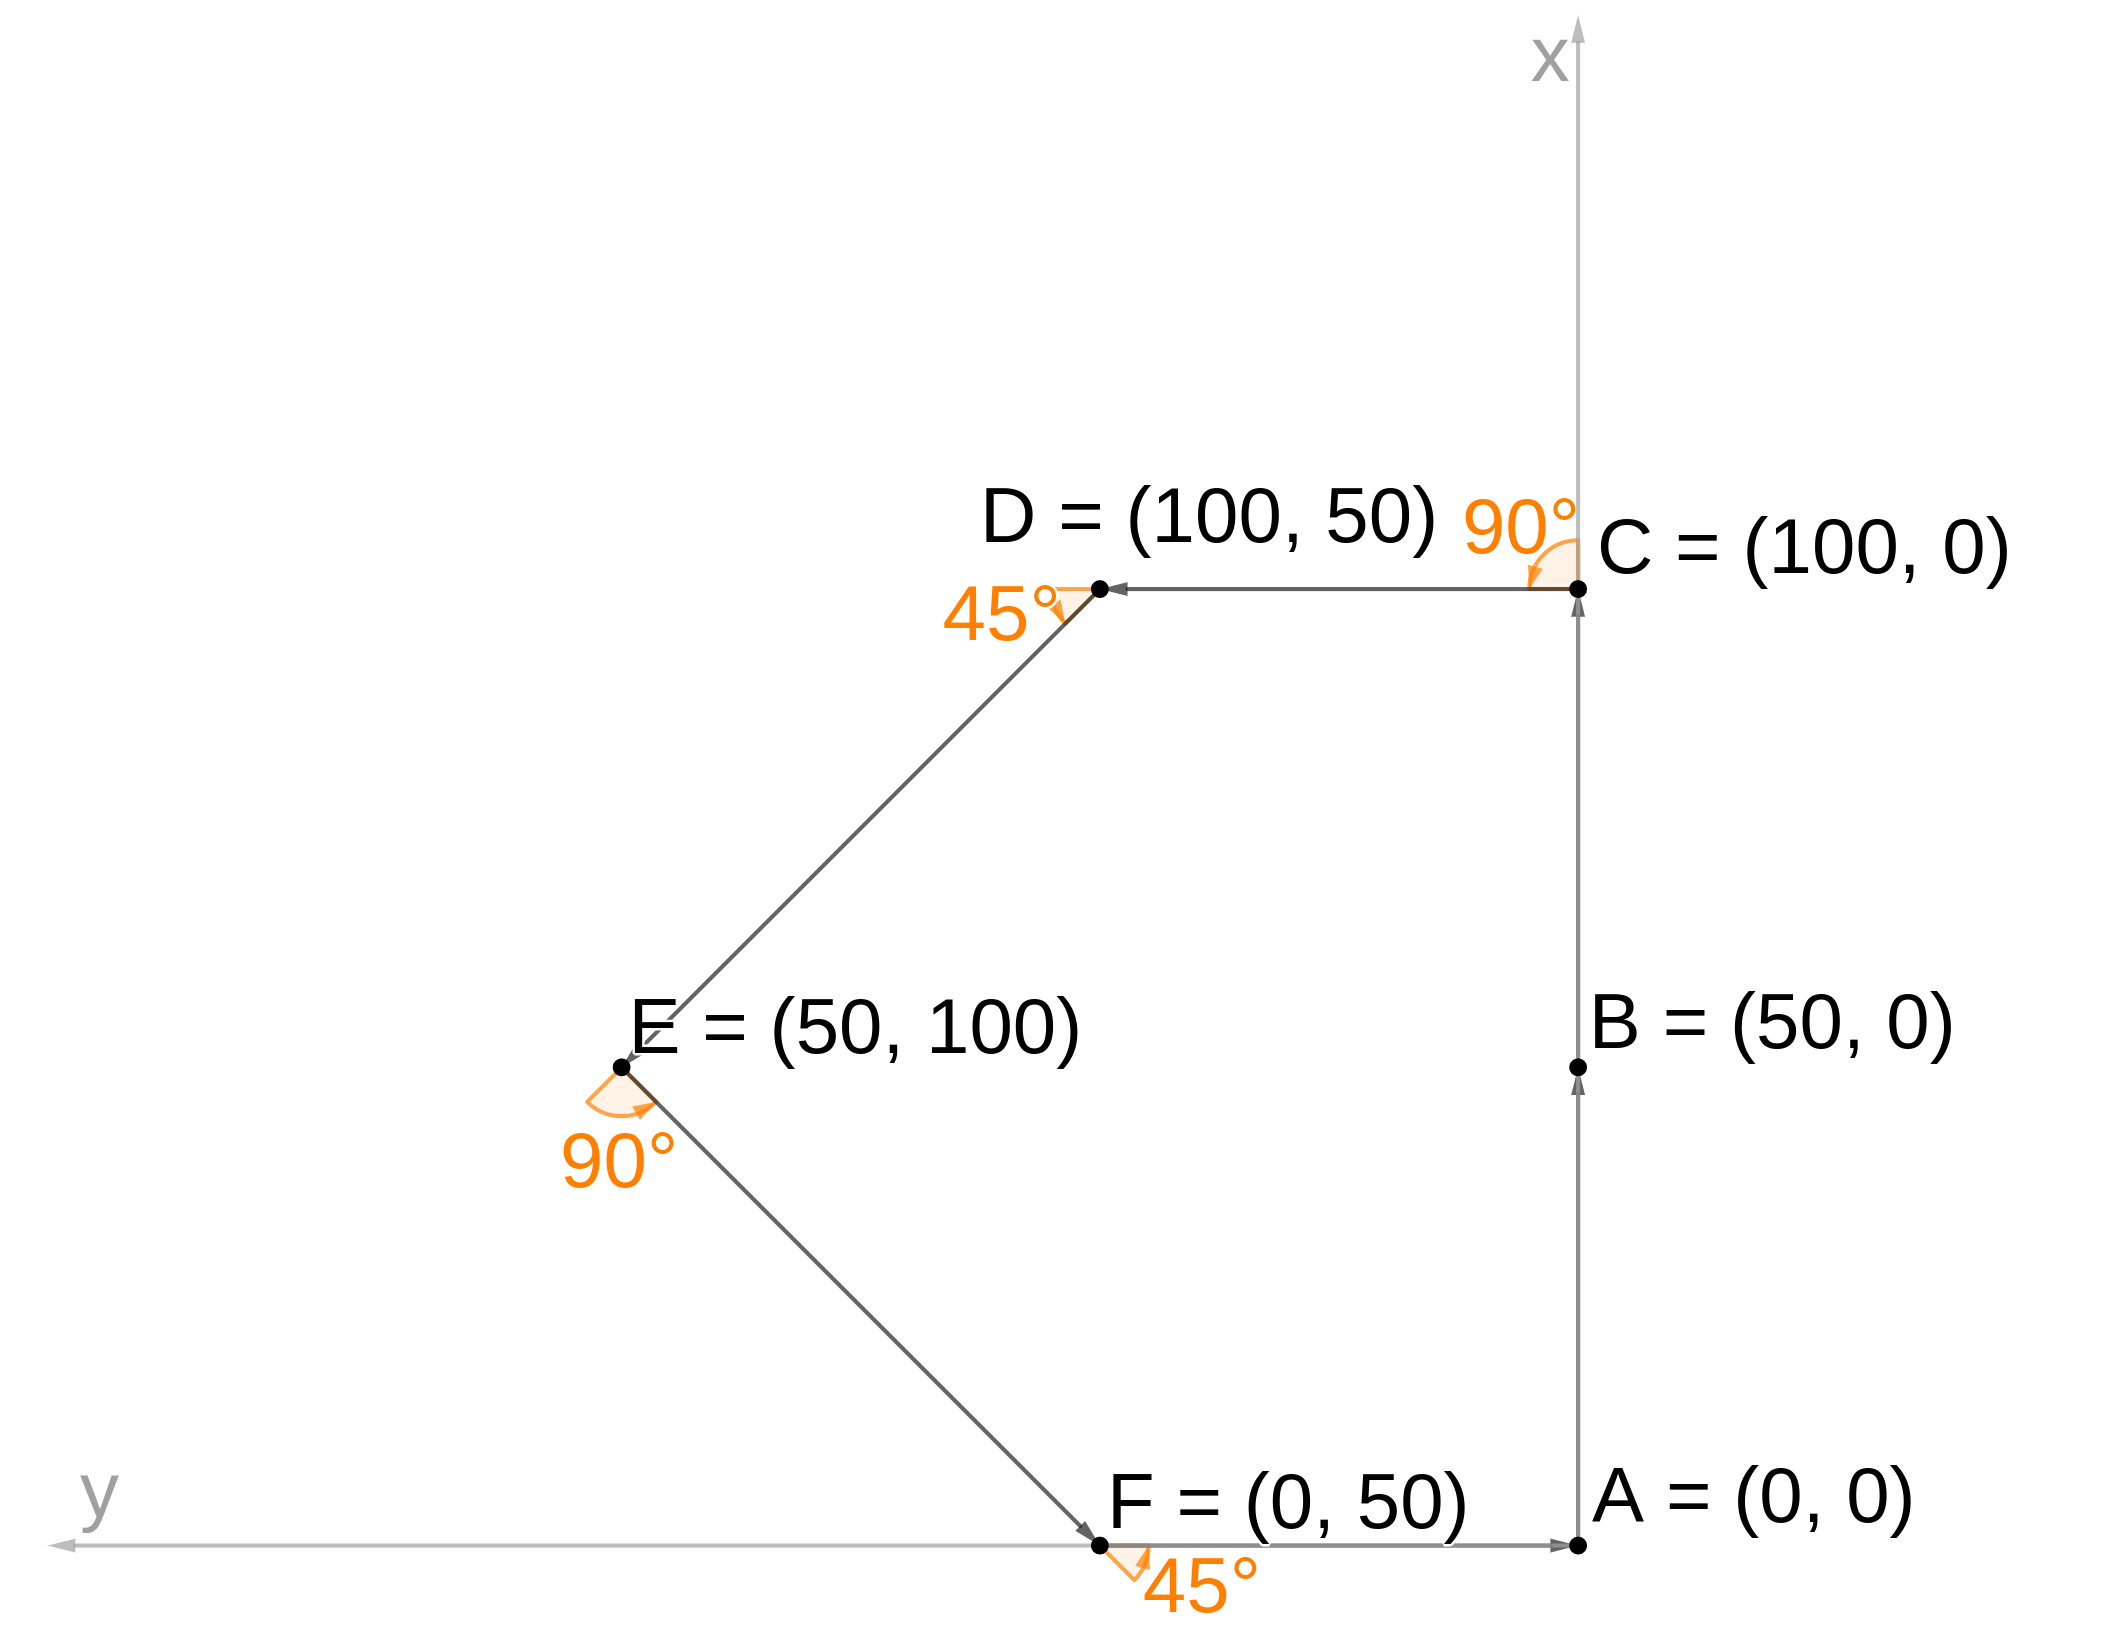
\includegraphics[scale=0.06]{test_path}
	\captionsetup{justification=centering, margin=1.5cm}
	\centering
	\caption{Expected trajectory for the test (distances are expressed in cm).}
	\centering
\end{figure}

\paragraph{Test 1}\mbox{}\\
\begin{figure}[!ht]
	\begin{subfigure}{0.35\textwidth}
		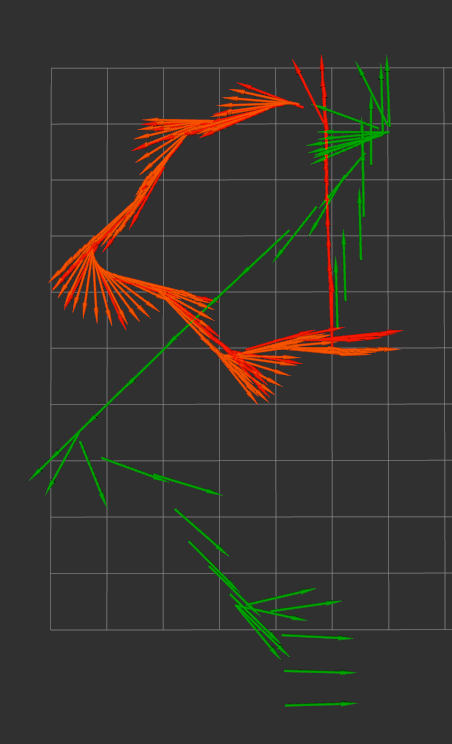
\includegraphics[width=\linewidth]{kf_test20}
	\end{subfigure}\hfil
	\begin{subfigure}{0.55\textwidth}
		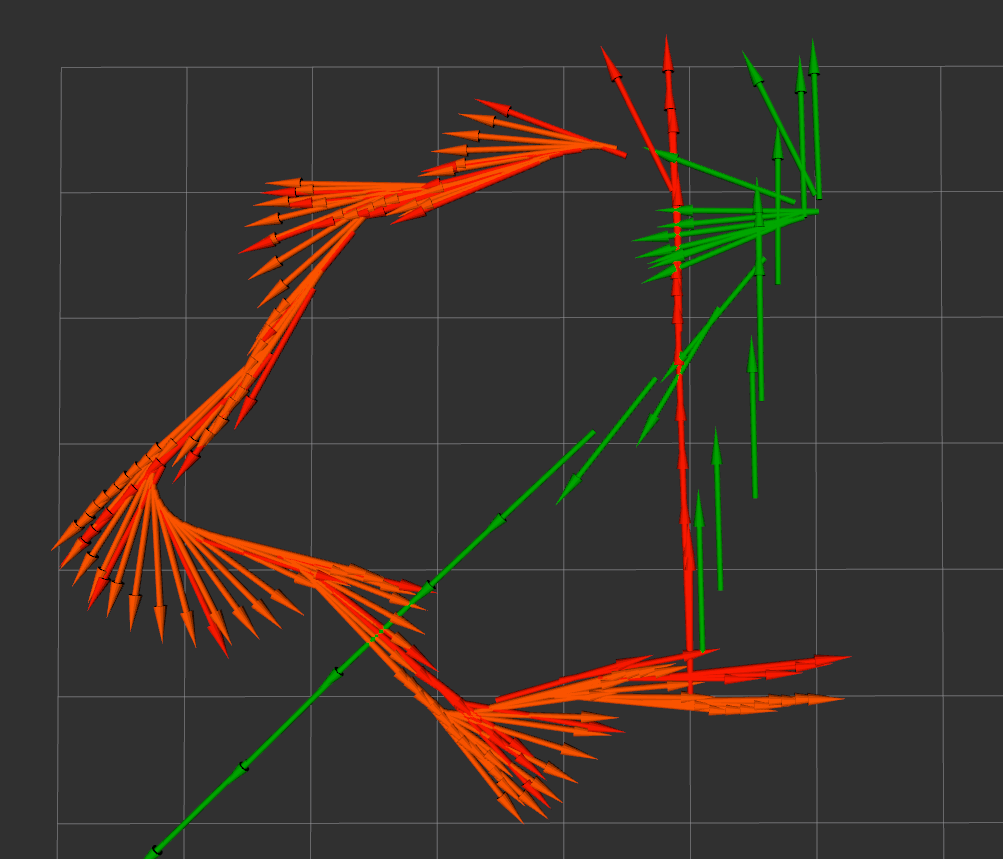
\includegraphics[width=\linewidth]{kf_test20_zoom}
	\end{subfigure}
	\captionsetup{justification=centering, margin=1.5cm}
	\centering
	\caption{Test 1 : estimated trajectories, Kalman filter trajectory in orange, Differential Drive trajectory in red, Inertial Navigation trajectory in green (visualized using RViz).}
	\centering
\end{figure}
\begin{table}[ht!]
	\centering
	\hspace*{-1cm}
	\begin{tabular}{rcccc}
		\toprule
		& \textbf{Expected} & \textbf{Kalman} & \textbf{Differential} & \textbf{Inertial}\\
		& \textbf{Position} & \textbf{Filter} & \textbf{Drive} & \textbf{Navigation}\\
		\midrule
		\textbf{A} & (0.000, 0.000, 0.000) & (0.000, 0.000, 0.000) & (0.000, 0.000, 0.000) & (0.000, 0.000, 0.000)\\
		\textbf{B} & (0.500, 0.000, 0.000) & (0.501, 0.009, 0.011) & (0.498, 0.016, 0.022) & (0.679, -0.141, 0.011)\\
		\textbf{C} & (1.000, 0.000, 0.000) & (1.002, 0.017, 0.010) & (0.999, 0.029, 0.011) & (0.991, -0.252, 0.010)\\
		\textbf{D} & (1.000, 0.500, 1.571) & (1.012, 0.523, 1.552) & (1.001, 0.534, 1.566) & (0.960, -0.256, 1.567)\\
		\textbf{E} & (0.500, 1.000, 2.356) & (0.509, 1.031, 2.325) & (0.481, 1.026, 2.349) & (-0.364, 1.117, 2.344)\\
		\textbf{F} & (0.000, 0.500, 3.927) & (-0.012, 0.518, 3.840) & (0.001, 0.479, 3.915) & (-1.136, 0.433, 3.866)\\
		\textbf{A} & (0.000, 0.000, 4.712) & (-0.009, 0.017, 4.721) & (0.046, -0.020, 4.807) & (-1.923, 0.205, 4.762)\\
		\bottomrule
	\end{tabular}
	\hspace*{-1cm}
	\caption{Test 1 : values for all the localization techniques [expressed as (x, y, theta)].}
\end{table}

By way of example we also report the final state\footnote{The state is expressed in the form $\begin{pmatrix}x & \dot{x} & \ddot{x} & y & \dot{y} & \ddot{y} & \theta & \dot{\theta}\\\end{pmatrix}\nonumber\\$} and covariance, calculated by the Kalman filter, at the end of the path after 60 seconds of motionless.
\begin{adjustwidth}{-0.6cm}{10pt}
	\begin{align}
		x &= \begin{pmatrix}
				-8.78e^{-3} & -1.14e^{-2} & -1.33e^{-2} & 1.67e^{-2} & 1.05e^{-2} & 1.24e^{-2} & 4.71 & -9.31e^{-4}\\
				\end{pmatrix}\nonumber\\
		\nonumber\\
		\Sigma_x &= \begin{pmatrix}
					2.67e^{-2} & 9.80e^{-5} & -2.37e^{-6} & 0 & 0 & 0 & 0 & 0\\
					9.80e^{-5} & 2.01e^{-4} & 2.34e^{-4} & 0 & 0 & 0 & 0 & 0\\
					-2.37e^{-6} & 2.34e^{-4} & 6.42e^{-4} & 0 & 0 & 0 & 0 & 0\\
					0 & 0 & 0 & 2.67e^{-2} & 1.00e^{-4} & 1.07e^{-8} & 0 & 0\\
					0 & 0 & 0 & 1.00e^{-4} & 2.06e^{-4} & 2.41e^{-4} & 0 & 0\\
					0 & 0 & 0 & 1.08e^{-8} & 2.41e^{-4} & 6.52e^{-4} & 0 & 0\\
					0 & 0 & 0 & 0 & 0 & 0 & 2.69e^{-7} & 2.51e^{-7}\\
					0 & 0 & 0 & 0 & 0 & 0 & 2.51e^{-7} & 5.01e^{-5}\\
				\end{pmatrix}\nonumber
	\end{align}
\end{adjustwidth}

\vspace{80pt}
\paragraph{Test 2}\mbox{}\\
\begin{figure}[!ht]
	\begin{subfigure}{0.35\textwidth}
		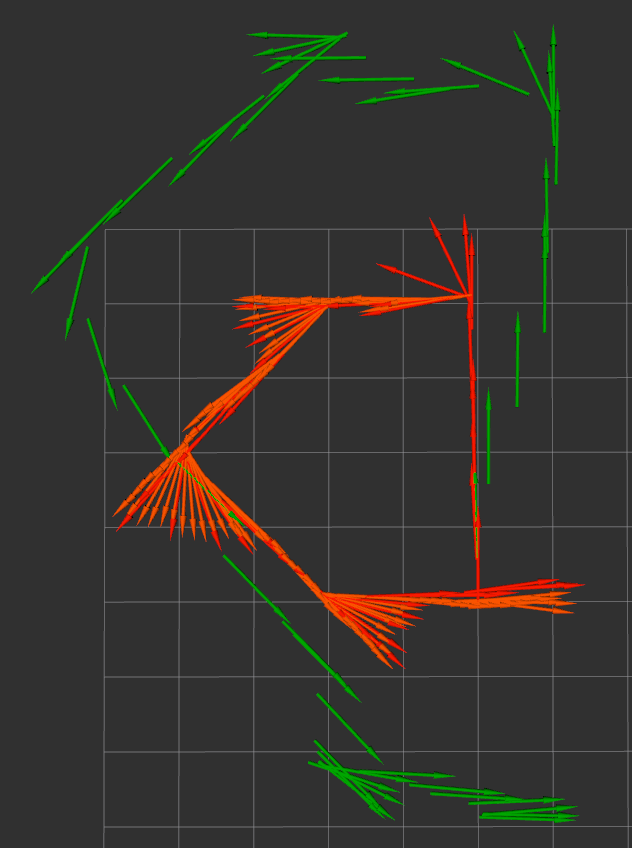
\includegraphics[width=\linewidth]{kf_test26}
	\end{subfigure}\hfil
	\begin{subfigure}{0.55\textwidth}
		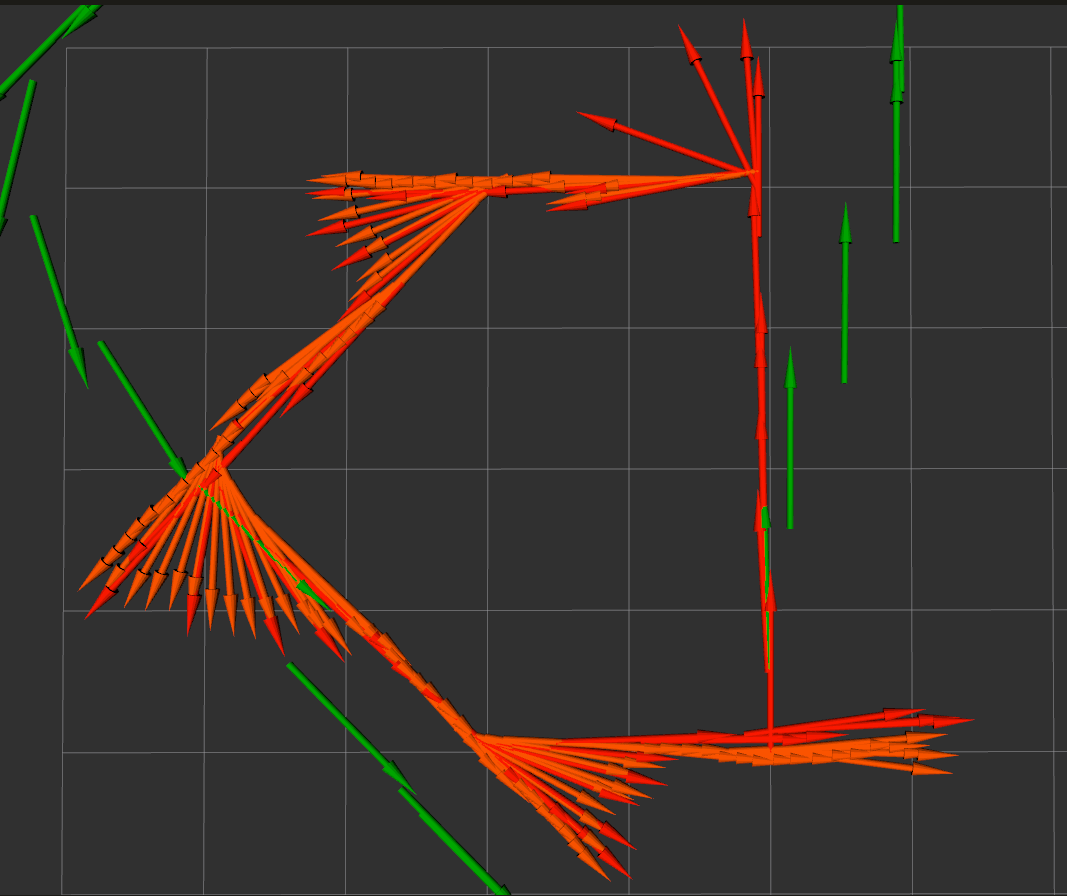
\includegraphics[width=\linewidth]{kf_test26_zoom}
	\end{subfigure}
	\captionsetup{justification=centering, margin=1.5cm}
	\centering
	\caption{Test 2 : estimated trajectories, Kalman filter trajectory in orange, Differential Drive trajectory in red, Inertial Navigation trajectory in green (visualized using RViz).}
	\centering
\end{figure}
\begin{table}[ht!]
	\centering
	\hspace*{-1.4cm}
	\begin{tabular}{rcccc}
		\toprule
		& \textbf{Expected} & \textbf{Kalman} & \textbf{Differential} & \textbf{Inertial}\\
		& \textbf{Position} & \textbf{Filter} & \textbf{Drive} & \textbf{Navigation}\\
		\midrule
		\textbf{A} & (0.000, 0.000, 0.000) & (0.000, 0.000, 0.000) & (0.000, 0.000, 0.000) & (0.000, 0.000, 0.000)\\
		\textbf{B} & (0.500, 0.000, 0.000) & (0.499, 0.000, 0.007) & (0.498, 0.012, 0.021) & (0.973, -0.224, -0.002)\\
		\textbf{C} & (1.000, 0.000, 0.000) & (1.001, 0.000, 0.006) & (0.980, 0.021, 0.076) & (1.528, -0.258, 0.056)\\
		\textbf{D} & (1.000, 0.500, 1.571) & (1.010, 0.501, 1.558) & (0.992, 0.502, 1.577) & (1.896, 0.455, 1.539)\\
		\textbf{E} & (0.500, 1.000, 2.356) & (0.516, 0.973, 2.348) & (0.524, 0.975, 2.367) & (-0.364, 1.117, 2.324)\\
		\textbf{F} & (0.000, 0.500, 3.927) & (0.006, 0.506, 3.906) & (-0.005, 0.481, 3.969) & (-0.516, 0.531, 3.911)\\
		\textbf{A} & (0.000, 0.000, 4.712) & (0.003, 0.000, 4.693) & (0.038, -0.025, 4.785) & (-0.707, -0.013, 4.691)\\
		\bottomrule
	\end{tabular}
	\hspace*{-1.4cm}
	\caption{Test 2 : values for all the localization techniques [expressed as (x, y, theta)].}
\end{table}
\newpage
By way of example we also report the final state and covariance, calculated by the Kalman filter, at the end of the path after 60 seconds of motionless.
\begin{adjustwidth}{-0.6cm}{10pt}
	\begin{align}
		x &= \begin{pmatrix}
				3.67e^{-3} & -3.57e^{-3} & -7.78e^{-3} & -2.38e^{-3} & 3.45e^{-3} & 7.69e^{-3} & 4.66 & 1.44e^{-4}\\
				\end{pmatrix}\nonumber\\
		\nonumber\\
		\Sigma_x &= \begin{pmatrix}
					1.31e^{-3} & 9.60e^{-6} & -8.84e^{-7} & 0 & 0 & 0 & 0 & 0\\
					9.60e^{-6} & 3.99e^{-5} & 8.70e^{-5} & 0 & 0 & 0 & 0 & 0\\
					-8.84e^{-7} & 8.70e^{-5} & 4.07e^{-4} & 0 & 0 & 0 & 0 & 0\\
					0 & 0 & 0 & 1.31e^{-3} & 9.60e^{6} & -8.84e^{-7} & 0 & 0\\
					0 & 0 & 0 & 9.60e^{-6} & 3.99e^{-5} & 8.70e^{-5} & 0 & 0\\
					0 & 0 & 0 & -8.84e^{-7} & 8.70e^{-5} & 6.52e^{-4} & 0 & 0\\
					0 & 0 & 0 & 0 & 0 & 0 & 1.31e^{-6} & 5.1e^{-9}\\
					0 & 0 & 0 & 0 & 0 & 0 & 5.1e^{-9} & 9.81e^{-7}\\
				\end{pmatrix}\nonumber
	\end{align}
\end{adjustwidth}
\vspace{80pt}
From these tests it emerges how the trajectory obtained with the sensor fusion (implemented through Kalman filtering) is surely far more accurate than the Inertial Navigation trajectory and it is also more accurate than the Differential Drive one. Moreover it also emerges how after a period of motionless the state is stable and the filter is very confident.\\



\begin{appendices}
	\chapter{Kalman Filter Implementation}\label{kf_implementation}

In this appendix we present the implementation of the Kalman filter.\\
Since all the Kalman filter is based on matrices, we needed to implement a few primitives to work with matrices and vectors which are presented in the first section. Then we will list the parameters and the global variables of the filter; and finally we wil show the Predict phase and the Update phase.\\

\section{Matrix Operations}
\begin{ccode}
	/* VECTORS */

	void vector_print(int size, float v[]);

	//adds two vectors of size len
	void vector_add(int len, float _a[], float _b[], float dest[]);

	//subtracts two vectors of size len
	void vector_sub(int len, float _a[], float _b[], float dest[]);

	/* MATRIXES */

	void matrix_print(int rows, int cols, float m[][cols]);

	//set to Identity matrix
	void matrix_set_identity(int size, float m[][size]);

	//calculates the transpose of matrix s
	void matrix_transpose(int rows, int cols, float s[][cols], float d[][rows]);

	//multiplies matrix per scalar value
	void matrix_scalar_mul(int rows, int cols, float m[][cols], float k, float d[][cols]);

	//adds two matrices
	void matrix_add(int rows, int cols, float _a[][cols], float _b[][cols], float dest[][cols]);

	//subtracts two matrices
	void matrix_sub(int rows, int cols, float _a[][cols], float _b[][cols], float dest[][cols]);

	//calculates the product of two square matrix
	void square_matrix_product(int size, float _left_m[][size], float _right_m[][size], float dest_m[][size]);

	//calculates the product of two general size matrix [left_m is r1 x c1, right_m is c1 x c2]
	void matrix_product(int r1, int c1, int c2, float left_m[][c1], float right_m[][c2], float dest_m[][c2]);

	//calculates the product of a matric and a vector
	void matrix_vector_product(int rows, int cols, float m[][cols], float _v[], float dest[]);

	//calculates the determinant of a matrix
	float matrix_determinant(int size, float m[][size]);

	//calculates the inverse of matrix m
	void matrix_inverse(int size, float m[][size], float inv[][size]);
\end{ccode}

\section{Parameters and Global Variables}
\begin{ccode}
	#define KF_ODOMETRY_UPDATE_RATE 100 // Hz
	float delta_time = 1./KF_ODOMETRY_UPDATE_RATE; //secs

	//covariance parameters
	#define PROCESS_NOISE_XY_COV 0.1 // m/s^3
	#define PROCESS_NOISE_THETA_COV 0.5 // rad/s^2

	#define OBSERV_IMU_ACCL_NOISE_COV 0.1
	#define OBSERV_IMU_GYRO_NOISE_COV 0.000001

	#define OBSERV_ENC_DXY_NOISE_COV 0.0000001
	#define OBSERV_ENC_DTHETA_NOISE_COV 0.000001


	//KF_STATUS
	#define KF_STATUS_LEN 8

	//KF_STATUS indexes following
	#define KF_ODOM_X 0
	#define KF_TRANS_VEL_X 1
	#define KF_TRANS_ACCL_X 2

	#define KF_ODOM_Y 3
	#define KF_TRANS_VEL_Y 4
	#define KF_TRANS_ACCL_Y 5

	#define KF_ODOM_THETA 6
	#define KF_ROT_VEL_Z 7


	//KF_OBSERVATION
	#define KF_OBSERVATION_LEN 6

	//KF_OBSERVATION indexes following
	#define KF_OBS_ENC_DX 0
	#define KF_OBS_ENC_DY 1
	#define KF_OBS_ENC_DTHETA 2

	#define KF_OBS_IMU_ACCL_X 3
	#define KF_OBS_IMU_ACCL_Y 4

	#define KF_OBS_IMU_ROTV_Z 5
	
	
	
	float dt = delta_time;
	float dt2_2 = .5*delta_time*delta_time;
	float dt3_6 = delta_time*delta_time*delta_time / 6.;
	
	//TRANSITION_MATRIX
	float TRANSITION_MATRIX[KF_STATUS_LEN][KF_STATUS_LEN] = 
		{{1.,dt,dt2_2,0.,0.,0.,0.,0.},
		{0.,1.,dt,0.,0.,0.,0.,0.},
		{0.,0.,1.,0.,0.,0.,0.,0.},
		{0.,0.,0.,1.,dt,dt2_2,0.,0.},
		{0.,0.,0.,0.,1.,dt,0.,0.},
		{0.,0.,0.,0.,0.,1.,0.,0.},
		{0.,0.,0.,0.,0.,0.,1.,dt},
		{0.,0.,0.,0.,0.,0.,0.,1.}};
	
	//TRANSITION_MATRIX_TRANSPOSE
	float TRANSITION_MATRIX_TRANSPOSE[KF_STATUS_LEN][KF_STATUS_LEN];
	matrix_transpose(KF_STATUS_LEN, KF_STATUS_LEN, TRANSITION_MATRIX, TRANSITION_MATRIX_TRANSPOSE);
	
	
	
	//transition noise will be modelled with 3 components:
		//[third_derivate_x, third_derivate_y, second_derivate_theta]
	#define TRANSITION_NOISE_LEN 3 //control covariance
	
		//PROCESS_NOISE_CONTRIBUTE_MATRIX
	float process_noise_covariance[TRANSITION_NOISE_LEN][TRANSITION_NOISE_LEN] =
			{{PROCESS_NOISE_XY_COV, 0., 0.},
			{0.,PROCESS_NOISE_XY_COV,0.},
			{0.,0.,PROCESS_NOISE_THETA_COV}};
	
	float transition_noise_matrix[KF_STATUS_LEN][TRANSITION_NOISE_LEN] = 
			{{dt3_6,0.,0.},
			{dt2_2,0.,0.},
			{dt,0.,0.},
			{0.,dt3_6,0.},
			{0.,dt2_2,0.},
			{0.,dt,0.},
			{0.,0.,dt2_2},
			{0.,0.,dt}};
	float transition_noise_matrix_transpose[TRANSITION_NOISE_LEN][KF_STATUS_LEN];
	matrix_transpose(KF_STATUS_LEN, TRANSITION_NOISE_LEN, transition_noise_matrix, transition_noise_matrix_transpose);
	
	float aux_cov[KF_STATUS_LEN][TRANSITION_NOISE_LEN];
	matrix_product(KF_STATUS_LEN, TRANSITION_NOISE_LEN, TRANSITION_NOISE_LEN, transition_noise_matrix, process_noise_covariance, aux_cov);
	float PROCESS_NOISE_CONTRIBUTE_MATRIX[KF_STATUS_LEN][KF_STATUS_LEN];
	matrix_product(KF_STATUS_LEN, TRANSITION_NOISE_LEN, KF_STATUS_LEN, aux_cov, transition_noise_matrix_transpose, PROCESS_NOISE_CONTRIBUTE_MATRIX);
	
	
	//OBSERVATION_COVARIANCE_MATRIX
	float OBSERVATION_COVARIANCE_MATRIX[KF_OBSERVATION_LEN][KF_OBSERVATION_LEN] =
		{{OBSERV_ENC_DXY_NOISE_COV,0.,0.,0.,0.,0.},
		{0.,OBSERV_ENC_DXY_NOISE_COV,0.,0.,0.,0.},
		{0.,0.,OBSERV_ENC_DTHETA_NOISE_COV,0.,0.,0.},
		{0.,0.,0.,OBSERV_IMU_ACCL_NOISE_COV,0.,0.},
		{0.,0.,0.,0.,OBSERV_IMU_ACCL_NOISE_COV,0.},
		{0.,0.,0.,0.,0.,OBSERV_IMU_GYRO_NOISE_COV}};
\end{ccode}
\captionof{lstlisting}{Parameters of the Kalman Filter}

\begin{ccode}
	//STATE
	float status_mean[KF_STATUS_LEN];
	float status_covariance[KF_STATUS_LEN][KF_STATUS_LEN];

	//OBSERVATION_MATRIX
	float observation_matrix[KF_OBSERVATION_LEN][KF_STATUS_LEN];
\end{ccode}
\captionof{lstlisting}{Global Variables of the Kalman Filter}

\section{Predict Phase}
\begin{ccode}
	//mean = A*mean
	matrix_vector_product(KF_STATUS_LEN, KF_STATUS_LEN, TRANSITION_MATRIX, status_mean, status_mean);
	
	//covariance = A*Cov*A_t
	square_matrix_product(KF_STATUS_LEN, TRANSITION_MATRIX, status_covariance, status_covariance);
	square_matrix_product(KF_STATUS_LEN, status_covariance, TRANSITION_MATRIX_TRANSPOSE, status_covariance);

	//covariance += B*Cov_noise*B_t
	matrix_add(KF_STATUS_LEN, KF_STATUS_LEN, status_covariance, PROCESS_NOISE_CONTRIBUTE_MATRIX, status_covariance);
\end{ccode}

\section{Update Phase}
\begin{ccode}
	//note: obs is an array of KF_OBSERVATION_LEN elements
	float obs[KF_OBSERVATION_LEN];
	obs[KF_OBS_ENC_DX] = sens_obs->local_dx;
	obs[KF_OBS_ENC_DY] = sens_obs->local_dy;
	obs[KF_OBS_ENC_DTHETA] = sens_obs->local_dtheta;
	obs[KF_OBS_IMU_ACCL_X] = sens_obs->imu_accel_x;
	obs[KF_OBS_IMU_ACCL_Y] = sens_obs->imu_accel_y;
	obs[KF_OBS_IMU_ROTV_Z] = sens_obs->imu_vel_theta;


	float sin_theta = sin(status_mean[KF_ODOM_THETA]);
	float cos_theta = cos(status_mean[KF_ODOM_THETA]);
	
	float dt2_2 = .5*delta_time*delta_time;
	float dt = delta_time;
	
	memset(&observation_matrix, 0, sizeof(observation_matrix));
	
	//ENCODERS
	observation_matrix[KF_OBS_ENC_DX][KF_TRANS_VEL_X] = cos_theta*dt;
	observation_matrix[KF_OBS_ENC_DX][KF_TRANS_ACCL_X] = cos_theta*dt2_2;
	observation_matrix[KF_OBS_ENC_DX][KF_TRANS_VEL_Y] = sin_theta*dt;
	observation_matrix[KF_OBS_ENC_DX][KF_TRANS_ACCL_Y] = sin_theta*dt2_2;
		
	observation_matrix[KF_OBS_ENC_DY][KF_TRANS_VEL_X] = -sin_theta*dt;
	observation_matrix[KF_OBS_ENC_DY][KF_TRANS_ACCL_X] = -sin_theta*dt2_2;
	observation_matrix[KF_OBS_ENC_DY][KF_TRANS_VEL_Y] = cos_theta*dt;
	observation_matrix[KF_OBS_ENC_DY][KF_TRANS_ACCL_Y] = cos_theta*dt2_2;
	
	observation_matrix[KF_OBS_ENC_DTHETA][KF_ROT_VEL_Z] = dt;
	
	
	// IMU
	//nel reference frame del robot:
		//	accel_x_local = accel_x_global * cos_theta + accel_y_global * sin_theta
		//	accel_y_local = -accel_x_global * sin_theta + accel_y_global * cos_theta
	observation_matrix[KF_OBS_IMU_ACCL_X][KF_TRANS_ACCL_X] = cos_theta;
	observation_matrix[KF_OBS_IMU_ACCL_X][KF_TRANS_ACCL_Y] = sin_theta;
	
	observation_matrix[KF_OBS_IMU_ACCL_Y][KF_TRANS_ACCL_X] = -sin_theta;
	observation_matrix[KF_OBS_IMU_ACCL_Y][KF_TRANS_ACCL_Y] = cos_theta;
	
	observation_matrix[KF_OBS_IMU_ROTV_Z][KF_ROT_VEL_Z] = 1.;
	
	//attended observation = C*status_mean
	float attended_obs[KF_OBSERVATION_LEN];
	matrix_vector_product(KF_OBSERVATION_LEN, KF_STATUS_LEN, observation_matrix, status_mean, attended_obs);	
	
	//K = cov_status*C_T * inverse(cov_noise + C*cov_status*C_T)
	float K_matrix[KF_STATUS_LEN][KF_OBSERVATION_LEN];
	
	float obs_matrix_transpose[KF_STATUS_LEN][KF_OBSERVATION_LEN];
	matrix_transpose(KF_OBSERVATION_LEN, KF_STATUS_LEN, observation_matrix, obs_matrix_transpose);	
	
	float aux_m_5_8[KF_OBSERVATION_LEN][KF_STATUS_LEN];
	matrix_product(KF_OBSERVATION_LEN, KF_STATUS_LEN, KF_STATUS_LEN, observation_matrix, status_covariance, aux_m_5_8);
	
	float aux_m_5_5[KF_OBSERVATION_LEN][KF_OBSERVATION_LEN];
	matrix_product(KF_OBSERVATION_LEN, KF_STATUS_LEN, KF_OBSERVATION_LEN, aux_m_5_8, obs_matrix_transpose, aux_m_5_5);
	
	matrix_add(KF_OBSERVATION_LEN, KF_OBSERVATION_LEN, OBSERVATION_COVARIANCE_MATRIX, aux_m_5_5, aux_m_5_5);
	
	matrix_inverse(KF_OBSERVATION_LEN, aux_m_5_5, aux_m_5_5);
	
	float aux_m_8_5[KF_STATUS_LEN][KF_OBSERVATION_LEN];
	matrix_product(KF_STATUS_LEN, KF_OBSERVATION_LEN, KF_OBSERVATION_LEN, obs_matrix_transpose, aux_m_5_5, aux_m_8_5);
	
	matrix_product(KF_STATUS_LEN, KF_STATUS_LEN, KF_OBSERVATION_LEN, status_covariance, aux_m_8_5, K_matrix);
	
	// status_mean += K_matrix * (obs - attended_obs)
	float delta_obs[KF_OBSERVATION_LEN];
	vector_sub(KF_OBSERVATION_LEN, obs, attended_obs, delta_obs);
	
	float delta_status[KF_STATUS_LEN];
	matrix_vector_product(KF_STATUS_LEN, KF_OBSERVATION_LEN, K_matrix, delta_obs, delta_status);
	
	vector_add(KF_STATUS_LEN, status_mean, delta_status, status_mean);
	
	//status_covariance -= (K_matrix*C ) * status_covariance
	float aux_m_8_8[KF_STATUS_LEN][KF_STATUS_LEN];
	matrix_product(KF_STATUS_LEN, KF_OBSERVATION_LEN, KF_STATUS_LEN, K_matrix, observation_matrix, aux_m_8_8);

	square_matrix_product(KF_STATUS_LEN, aux_m_8_8, status_covariance, aux_m_8_8);

	matrix_sub(KF_STATUS_LEN, KF_STATUS_LEN, status_covariance, aux_m_8_8, status_covariance);
\end{ccode}

\end{appendices}
\backmatter

\cleardoublepage

\phantomsection

%\bibliographystyle{sapthesis} % BibTeX style
\printbibliography[title=References,heading=bibintoc]

\end{document}
